
\section{rANS}
    \subsection{Key Concepts}
    \begin{frame}[fragile]{rANS}
        \begin{itemize}
            \item "r" = "range": similar to range coding (RC)
            \item symbol spread function
            \item representation of information
            \item asymmetric
        \end{itemize}
    \end{frame}

    \subsection{Exa. 3}
    \begin{frame}[fragile]{Exa.3}
        How to encode 101110? What is the encoding function $C(s,x)$? \ $x' = C(s,x) \approx x/p_s$
    \end{frame}
    \begin{frame}[plain]
        \begin{figure}
            \centering
            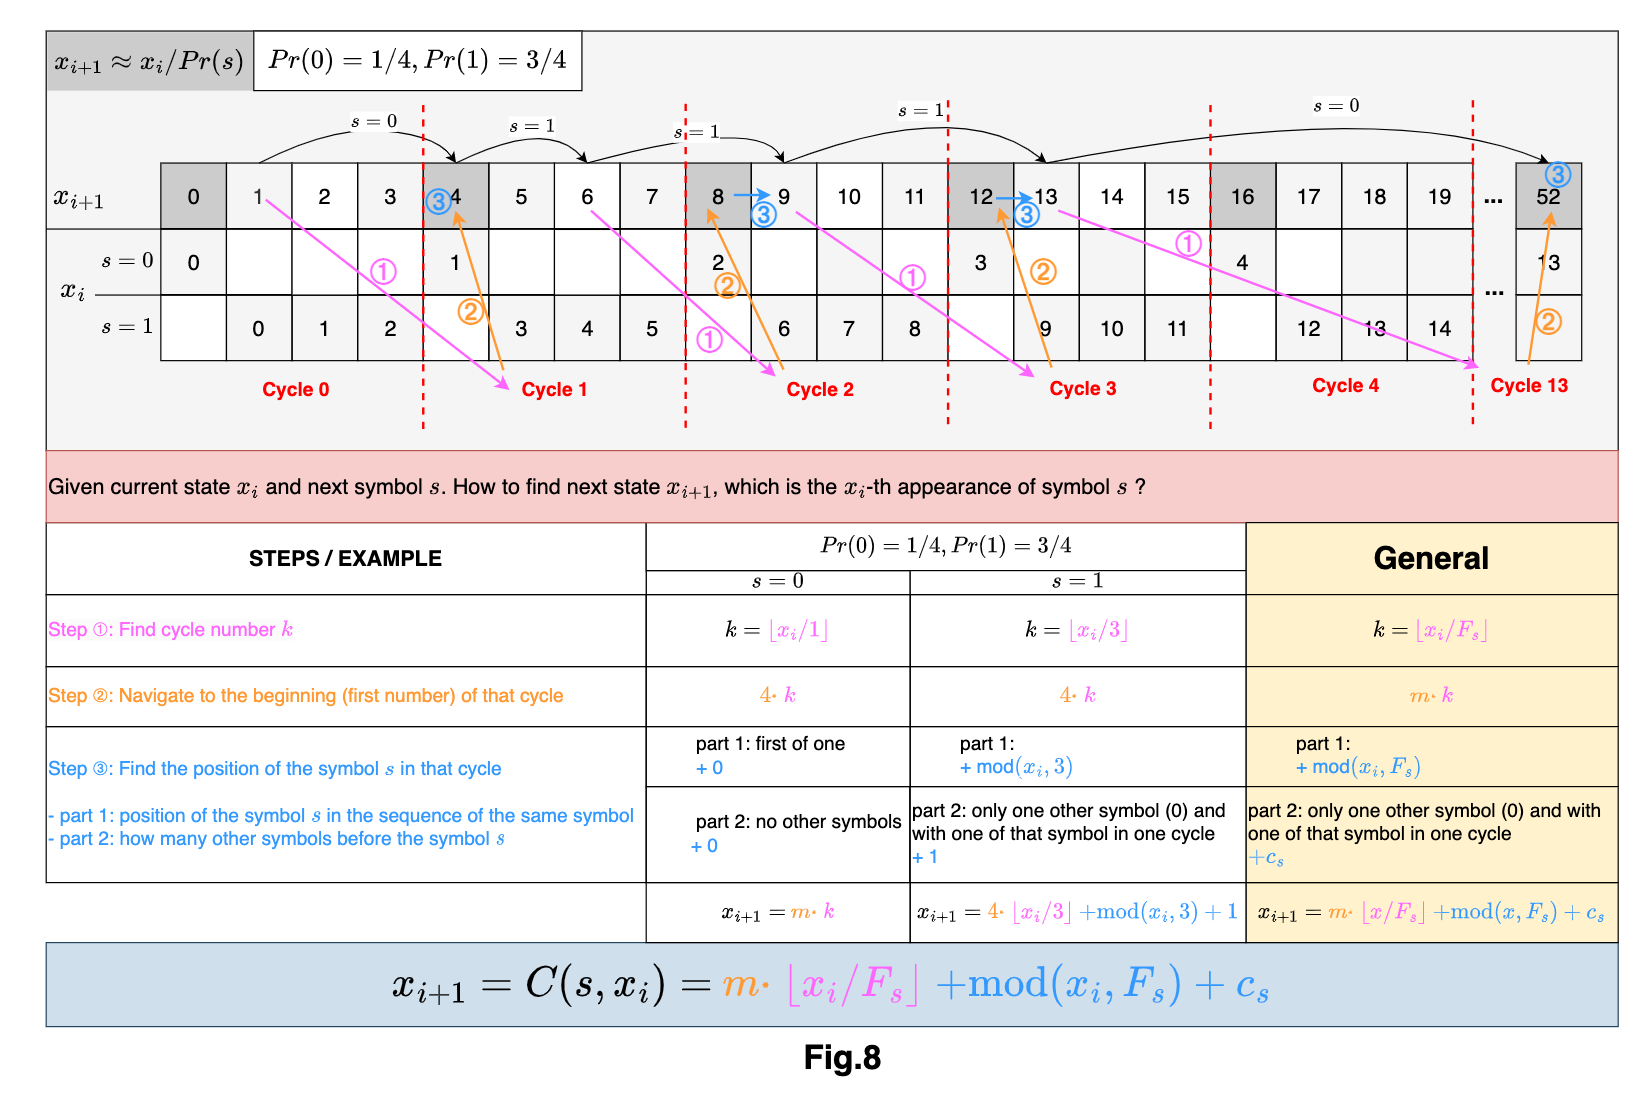
\includegraphics[width=1\textwidth,height=1.07\textheight,keepaspectratio]{../24ws_ANS.assets/fig8.png}
        \end{figure}
    \end{frame}

    \subsection{Encoding Function}
    \begin{frame}[fragile]{}
        \textbf{Encoding Function \refer{2} \refer{5}:}
        \[
        x' = m \cdot \left\lfloor x/F_s \right\rfloor + \operatorname{mod}(x, F_s) + c_s 
        \]
        \begin{itemize}
            \item \textbf{Alphabet set:} \(\mathcal{A} = \{a_1, a_2, \dots, a_k\}\)
            \item \textbf{Absolute frequency of symbol \(s\):} \(F_s\)
            \item \textbf{Total frequency:} $m = \sum_{i=1}^{k} F_i$
            \item \textbf{Probability of symbol \(s\):} $p_s = \frac{F_s}{m}$
            \item \textbf{Cumulative frequency before \(s\):} $c_s := F_0 + F_1 + \dots + F_{s-1}$
            % \item \textbf{Input sequence:} 
            % \[
            % S_{\text{in}} = (s_1, s_2, \dots, s_n)
            % \]
        \end{itemize}
    \end{frame}

    \begin{frame}[fragile]{}
        \textbf{Encoding Function (binary) \refer{2} : maybe no need to put this slide, let's see}
        \[
        x' = C(s,x) = \left\lfloor x/F_s \right\rfloor << n+ \operatorname{mod}(x, F_s) + c_s \, 
        \]
        \begin{itemize}
            \item \textbf{Alphabet set:} \(\mathcal{A} = \{a_1, a_2, \dots, a_k\}\)
            \item \textbf{Absolute frequency of symbol \(s\):} \(F_s\)
            \item \textbf{Total frequency:} $m = \sum_{i=1}^{k} F_i$
            \item \textbf{Probability of symbol \(s\):} $p_s = \frac{F_s}{m}$
            \item \textbf{Cumulative frequency before \(s\):} $c_s := F_0 + F_1 + \dots + F_{s-1}$
            \item $<< n$ is a left shift by $n$ bits
            % \item \textbf{Input sequence:} 
            % \[
            % S_{\text{in}} = (s_1, s_2, \dots, s_n)
            % \]
        \end{itemize}
    \end{frame}


    \subsection{Decoding Function}
    \begin{frame}[plain]
        \begin{figure}
            \centering
            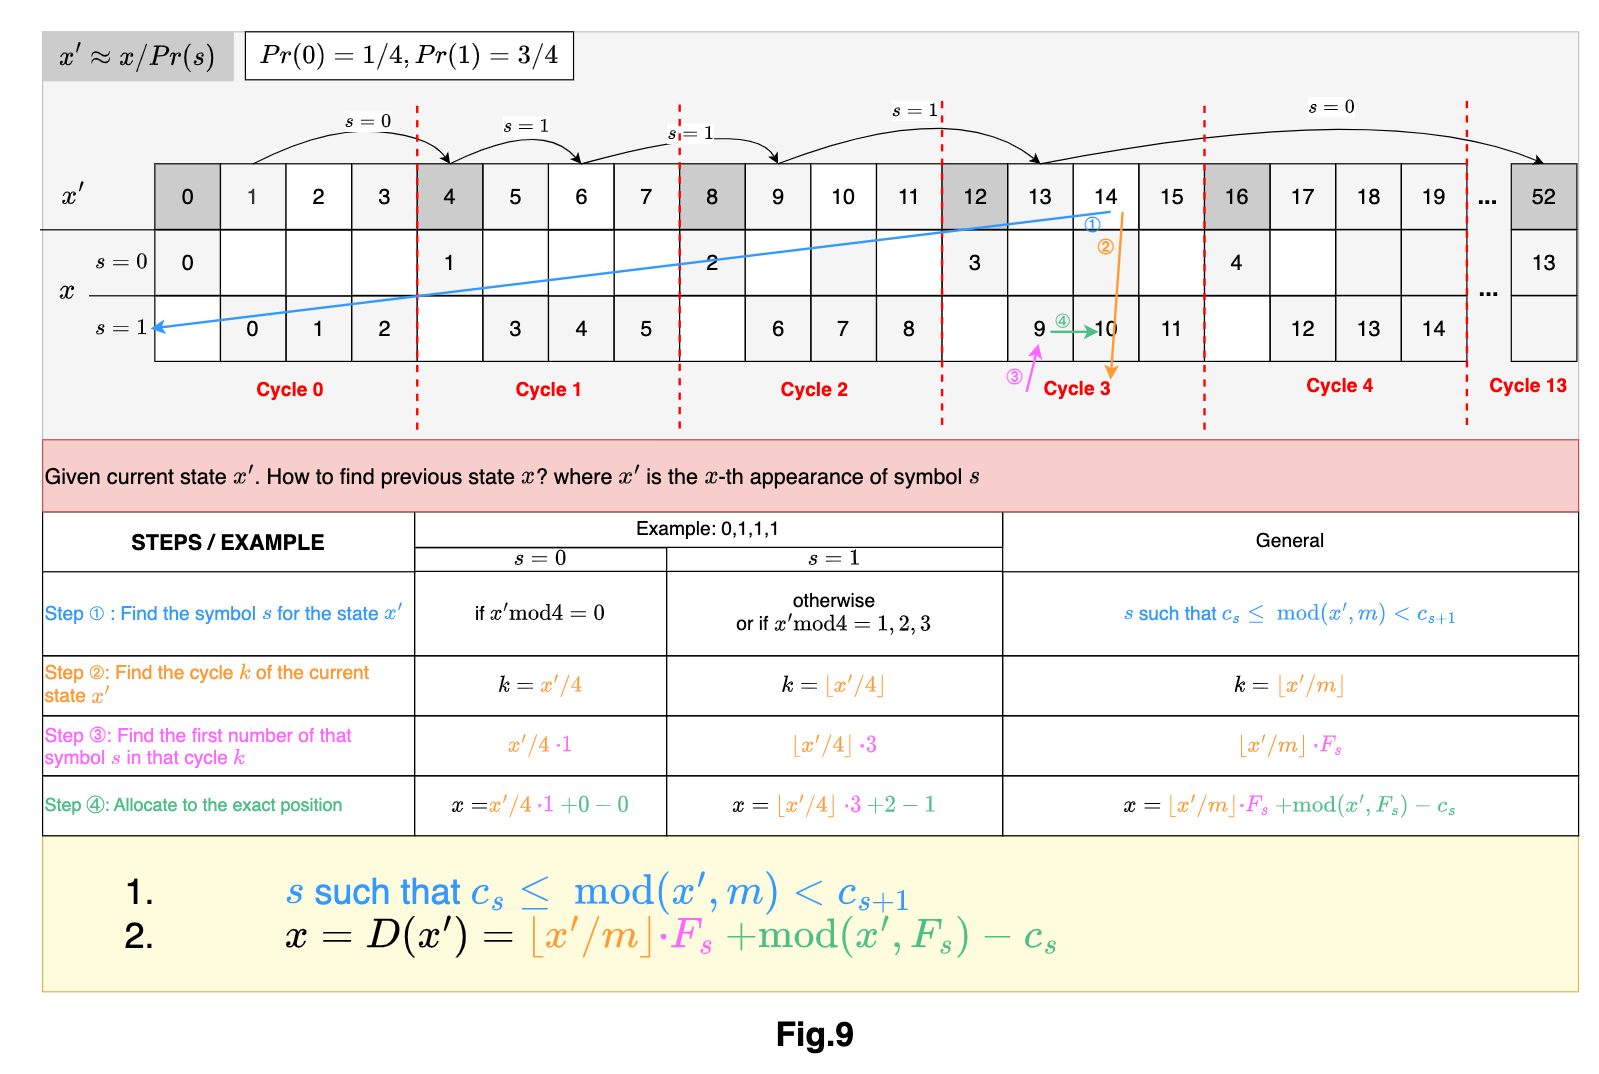
\includegraphics[width=1\textwidth,height=1.07\textheight,keepaspectratio]{../24ws_ANS.assets/fig9.png}
        \end{figure}
    \end{frame}
    \begin{frame}
        \textbf{Decoding Function (binary):}
        \[
        D(x) = (s, F_s \cdot (x >> n)+ (x \& mask) - c_s) \refer{2}
        \]
        \begin{itemize}
            \item 
        \end{itemize}
    \end{frame}

    \subsection{Implementation}
    \subsubsection{Encoding}
    \begin{frame}[fragile]{}
        \begin{minted}[fontsize=\scriptsize, linenos, breaklines]{python}
            def rANS_encoder(symbol_counts, s_input):
                # compute cumulative frequencies
                cumul_counts = []
                sum_counts = 0
                for count in symbol_counts:
                    cumul_counts.append(sum_counts)
                    sum_counts += count
                state = 0
                output = []
                for s in s_input:
                    Fs = symbol_counts[s]
                    Cs = cumul_counts[s]
                    state = (state // Fs) * sum_counts + Cs + (state % Fs)
                    output.append((s, state))
                
                L_avg = math.ceil(math.log(state) / math.log(2.0)) / len(s_input)
                return output, state, L_avg, entropy(symbol_counts)
        \end{minted}
        \href{http://localhost:8050}{Implemenation in Dash app with interactive visualization}
    \end{frame}
    \subsubsection{Decoding}
    \begin{frame}[fragile]{}
        \begin{minted}[fontsize=\scriptsize, linenos, breaklines]{python}
            def rANS_decoder(symbol_counts, num_symbols, state):
                cumul_counts = [0]  # Start with 0 as the first cumulative frequency
                total_frequency = sum(symbol_counts)
                for count in symbol_counts:
                    cumul_counts.append(cumul_counts[-1] + count)
                def c_inv(y):
                    return bisect_right(cumul_counts, y) - 1
                output = []  # List to store decoded symbols
                for _ in range(num_symbols):
                    slot = state % total_frequency  # Find the slot in the cumulative frequency range
                    s = c_inv(slot)                 # Get the symbol corresponding to the slot
                    Fs = symbol_counts[s]           # Frequency of the symbol
                    Cs = cumul_counts[s]            # Cumulative count of the symbol
                    output.append((s,state))                # Append decoded symbol to the output
                    state = (state // total_frequency) * Fs + (slot - Cs)  # Update the state
                return output, state
        \end{minted}
        \href{http://localhost:8050}{Implemenation in Dash app with interactive visualization}
    \end{frame}
